\documentclass[a4paper]{article}
\usepackage{hyperref}
\usepackage{graphicx}

\begin{document}
	\title{Project LevelGen - User Guide}
	\author{Mikael R Hanssen}
	\maketitle
	
	\tableofcontents
	\newpage
	
	\section{Getting Started}
	\subsection{Installing LevelGen}
	Download the latest version of LevelGen (currently hosted a \url{https://github.com/Xhine0/LevelGen}), and place the folder somewhere in your project's assets folder.
	\subsection{Setting up the level generator}
	Open the LevelGen graph and inspector, by clicking 'Level Generator $\rightarrow$ Show all' in the toolbar. 
	\\First, a level generator must exist in the scene. To create one, Click 'Create' in the 'Room Inspector'. An object named '\_Level' should appear in the scene.
	\subsection{Setting up a level}
	First, a level save file must be created. This is done by right-clicking in the 'Project' window, then select 'Create $\rightarrow$ Level'. A file named 'New Level' should now appear. 
	\\ To edit the level, add it to the level field in the room inspector.
	
	\section{LevelGen Manual}
	\subsection{Rooms}
	A room is defined by a bit map, where each pixel color represents a unique object, called a block. Each room can have one or more exits.
	\subsubsection{Blocks}
	A block is simply a prefab, defined by the user, that is represented by a unique color in the room's bit map.
	\subsubsection{Exits}
	An exit is a special block that connects one or more rooms together. All exits of one room can be connected to any exit of the other rooms.
	
	\newpage
	
	\section{Using the LevelGen GUI}
	\subsection{Managing rooms}
	\subsubsection{Creating a room}
	In the room inspector, click the 'Create Room' button, located at the bottom. The following menu (figure \ref{fig:create_room}) will appear:
	
	\begin{figure}[h]
		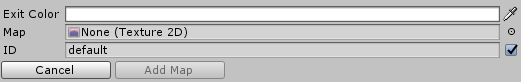
\includegraphics[width=\linewidth]{img/Menu_CreateRoom.PNG}
		\caption{The room creation panel}
		\label{fig:create_room}
	\end{figure}

	The exit color defines where the room's exits are placed. 
	\\When a bit map and an available id is assigned, the room can be created by clicking 'Add Room'. The room should now appear as a node on the room graph (figure \ref{fig:node_room})
	
	\subsubsection{Editing a room}
	\begin{figure}[h]
		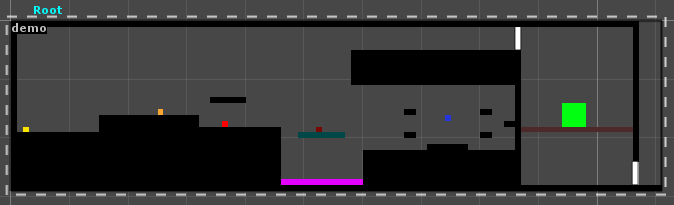
\includegraphics[width=\linewidth]{img/Node_Room.PNG}
		\caption{A node in the room graph}
		\label{fig:node_room}
	\end{figure}
	
	\begin{figure}[h]
		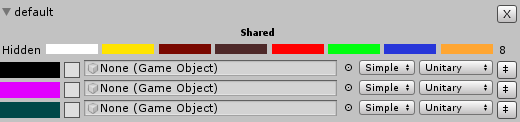
\includegraphics[width=\linewidth]{img/Menu_EditRoom.PNG}
		\caption{Room editing}
		\label{fig:edit_room}
	\end{figure}
	
	To edit a room, it must first be selected in the room graph. It should now appear in the room inspector (figure \ref{fig:edit_room}). 
	
	\subsubsection{Editing blocks}
	To add a block entry to the selected room, click on the desired color in the room's block list. Click on the color of an existing entry to remove it.  
\end{document}